%************************************************
\chapter{Theoretical Framework}\label{ch:relatedwork}
%************************************************

\section{Eligibility Propagation}

    \subsection{Network model}
        An eligibility propagation model $\mathcal{M}$ is defined by a tuple $\left<M, f\right>$,
        where $M$ is a function
        \begin{equation}\label{eq:model}
        \mathbf{h}^t_j = M\left(\mathbf{h}_j^{t-1}, \mathbf{z}^{t-1}, \mathbf{x}^t, \mathbf{W}_j\right)
        \end{equation}
        that defines the hidden state $\mathbf{h}_j^t$ of a neuron $j$ at a discrete time step $t$, where $\mathbf{z}^{t-1}$ is the observable state of all neurons at the previous time step (\ie, the binary spike values), $\mathbf{x}^t$ is the model input vector at time $t$, and $\mathbf{W}_j$ is the weight vector of afferent synapses.
        The update of the observable state of a neuron $j$ at time $t$ is defined by
        \begin{equation}
        z^t_j = f\left(\mathbf{h}_j^t\right).
        \end{equation}
        This formalization means that e-prop is a \emph{local} training method, because a neuron's observable state depends only on its own hidden state, and the hidden state depends only on observable signals that are directly connected to it.
        E-prop is also an \emph{online} training method, because both the hidden and observable state of a neuron depend only on variables in the previous time point.

    \subsection{Neuron models}\label{sec:alif}

        \paragraph{LIF neuron}
            In \citet{bellec2020solution}, the LIF neuron model is formulated in the context of e-prop, along with a variant (viz. ALIF) that has an adaptive threshold based on the neuron's spiking frequency.
            The observable state of a LIF model is given by
            \begin{equation}
            z^t_j = H\left(v_j^t-v_\text{th}\right),
            \end{equation}
            where $H$ is the Heaviside step function, and $v_\text{th}$ is the threshold constant.
            (Note that this and all other used constant parameters are listed in Table \ref{tab:hparams}.)
            Consequently, the observable state $z^t_j \in \{0, 1\}$ is binary, and denotes the spike activity of a neuron.
            These spikes are the only communication between neurons in the model.
            The LIF neuron model has a single state $h^t_j$ that contains only an activity value $v^t_j$ and evolves over time according to the equation
            \begin{equation}\label{eq:alifV}
            v^{t+1}_j = \alpha v_j^t + \sum_{i\neq j}W^\text{rec}_{ji}z_i^t + \sum_i W^\text{in}_{ji}x_i^{t+1} - z_j^tv_
            \text{th},
            \end{equation}
            where $W^\text{rec}_{ji}$ is a synapse weight from neuron $i$ to neuron $j$, $\alpha$ is a constant decay factor.
            Whenever $j$ spikes (i.e., $z_j^t = 1$), the activity of the neuron is reduced to a value near 0 by the term $-z^t_jv_\text{th}$.
            Furthermore, $z^t_j$ is fixed to 0 for $T^\text{refr}$ time steps to model neuronal refractoriness.
            In biological neurons, the refractory period consists of an ``absolute'' phase, during which evoking a new spike is impossible, and a subsequent ``relative'' phase where the threshold is temporarily increased \citep{purves2008neuroscience}.
            Clamping $z^t_j$ to 0 emulates only this absolute phase.


        \paragraph{ALIF neuron}
            The ALIF neuron introduces a threshold adaptation variable $a^t_j$ to the hidden state of the neuron, such that $\mathbf{h}^t_j \eqdef \left[v^t_j, a^t_j\right]$.
            In an ALIF neuron, the spiking threshold increases after a spike, and otherwise decreases back to a baseline threshold $v_\text{th}$.

            This resembles \emph{spike frequency adaptation} (SFA), a common feature of neocortical pyramidal neurons \citep{benda2003universal}.
            SFA is a homeostatic control mechanism that affects the spiking frequency based on the recent spiking activity.
            \citet{ahmed1998estimates} found that a single time constant is a good fit to characterize the threshold's exponential decay to a steady state.

            The observable state of an ALIF neuron is therefore described by
            \begin{equation}\label{eq:alifZ}
            z^t_j = H\left(v_j^t - v_\text{th} - \beta a^t_j\right)
            \end{equation}
            and
            \begin{equation}\label{eq:alifA}
            a^{t+1}_j = \rho a^t_j + z^t_j,
            \end{equation}
            where $\rho$ is an adaptation decay constant.
            The interaction between the neuron activity, adaptive threshold and spiking behavior is illustrated in Figure \ref{fig:simplealif}.

            \begin{figure}[!ht]
                \centering
                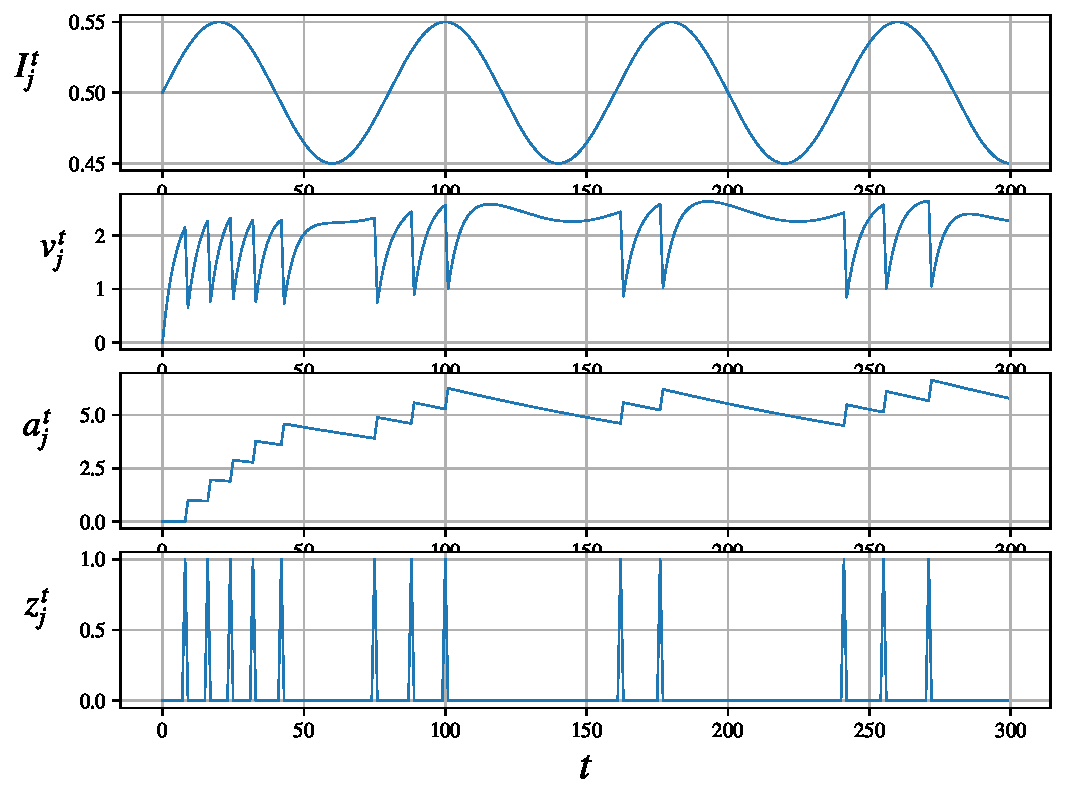
\includegraphics[width=\linewidth]{gfx/simplealif}
                \caption[ALIF neuron simulation.]{A simulated ALIF neuron $j$ receives a sinusoidal input $I$ for 300 time steps $t$. This figure illustrates the adaptive threshold $a$, which increases at every spike $z$, requiring a higher activity $v$ for a next spike. When a spike occurs, $v$ decreases by $v_\text{th}$.}
                \label{fig:simplealif}
            \end{figure}

            In this paper, the LIF neuron is generalized as an ALIF neuron for which $\beta=0$, effectively canceling the effect of the threshold adaptation value $a^t_j$ on the observable state $z^t_j$ in Equation \ref{eq:alifZ}.
            Therefore, only the e-prop derivations for the ALIF neurons will be described in the following sections.

    \subsection{Network topology}

        The neurons receive inputs from the input feature vector and the observable states of the afferent neurons.

        Weights are initialized by sampling them from a Gaussian distribution $\mathcal{N}\left(0, \sqrt{N}\right)$ where $N$ is the number of afferent neurons.
        For instance, the weights $\mathbf{W}^\text{in}$ between the input and the first layer are sampled from $\mathcal{N}\left(0, \sqrt{39}\right)$, because there are 39 input features.

        A randomly selected 80\% of synaptic weights is then set to a value of 0, as well as the synapses that connect a neuron to itself, rendering them ineffective.

        Figure \ref{fig:topology-sl} illustrates the basic architecture of a single-layer e-prop model.
        \begin{figure}[!ht]
            \myfloatalign
            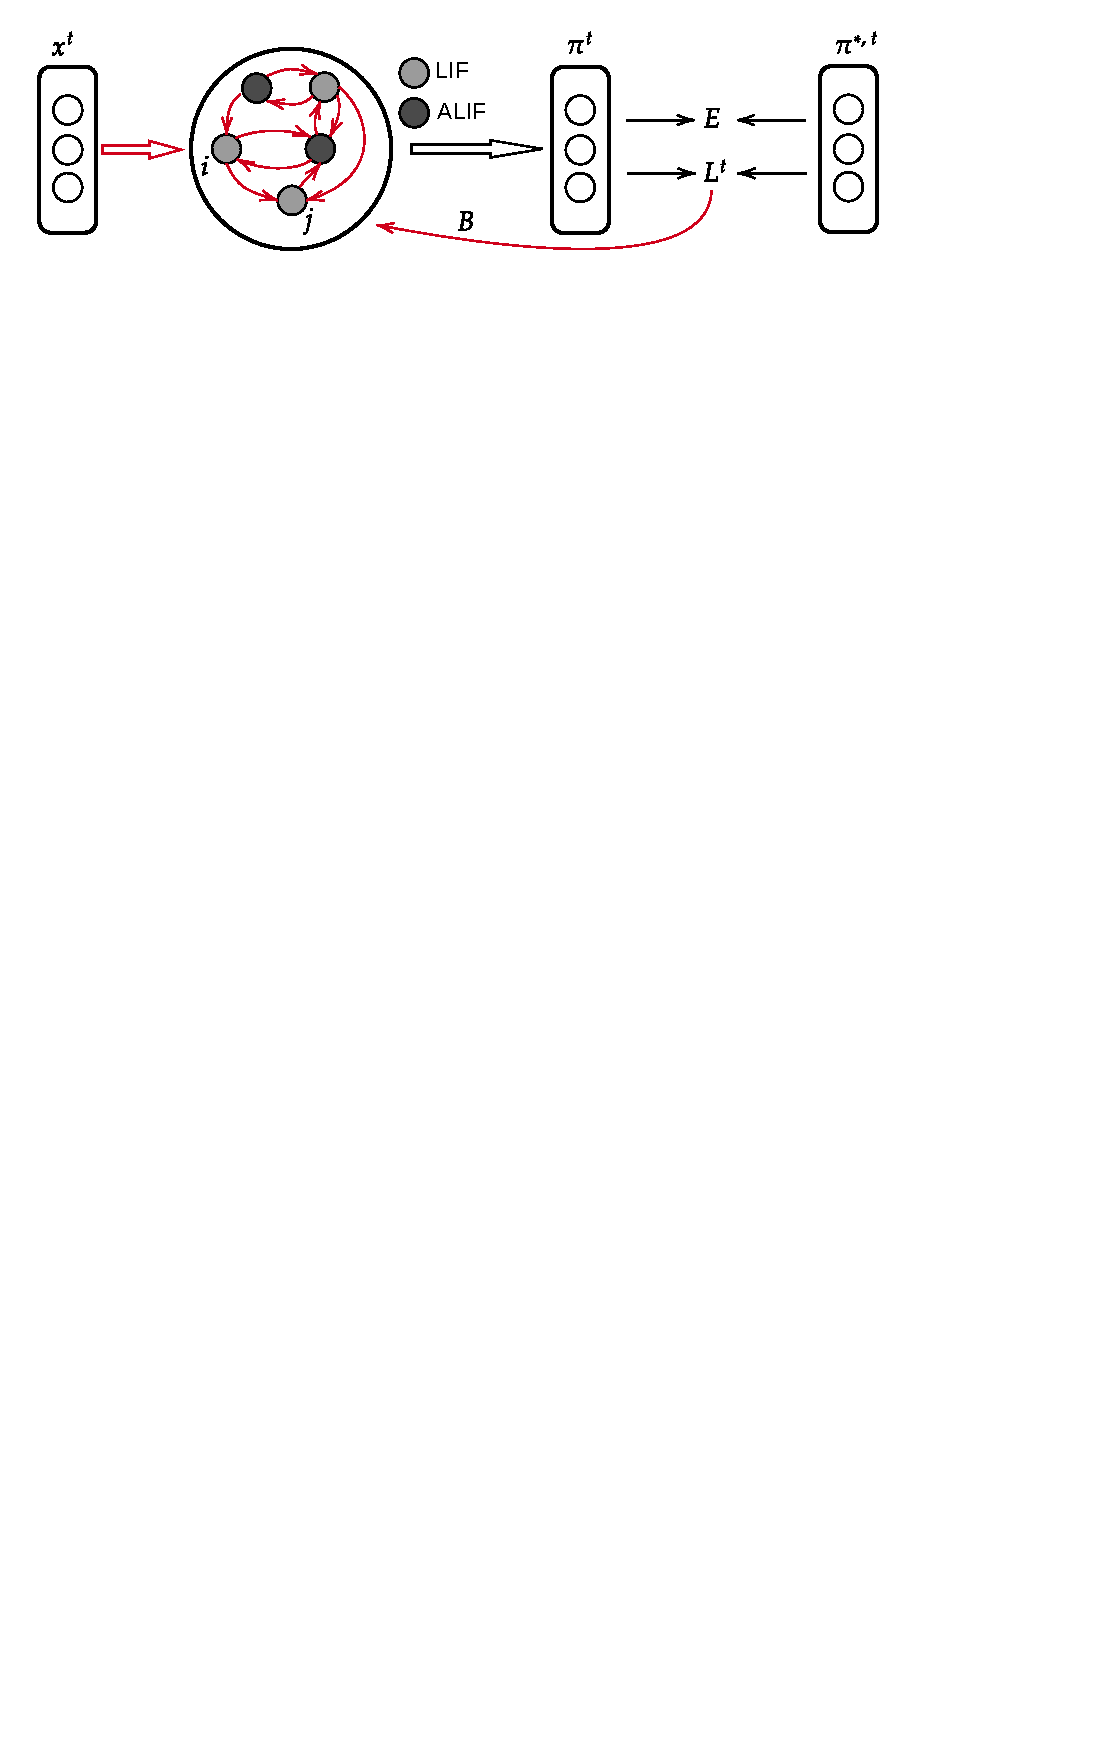
\includegraphics[trim=0 25cm 0 0, clip, width=\linewidth]{gfx/Singlelayer}
            \caption[Multi-layer illustration.]{An illustration of a single-layer network architecture.}
            \label{fig:topology-sl}
          \end{figure}


    \subsection{Deriving e-prop from RNNs}\label{sec:derivefromBPTT}
        Eligibility propagation is a local and online training method that can be derived from backpropagation through time (BPTT).
        In BPTT, an RNN is unfolded in time, such that the backpropagation method used in feedforward neural networks can be applied to compute the gradients of the cost with respect to the network weights.

        In this subsection, the main equation of e-prop
        \begin{equation}
        \frac{dE}{dW_{ji}} =
        \sum_t\frac{dE}{dz_j^t}\cdot\left[\frac{dz_j^t}{dW_{ji}}\right]_\text{local}
        \end{equation}
        is derived from the classical factorization of the loss gradients in an unfolded RNN:
        \begin{equation}\label{eq:clafac}
        \frac{dE}{dW_{ji}} = \sum_{t'}\frac{dE}{d\mathbf{h}_j^{t'}}\cdot\frac{\partial \mathbf{h}_j^{t'}}{\partial W_{ji}},
        \end{equation}
        where summation indicates that weights are shared.

        We now decompose the first term into a series of learning signals $L_j^t = \frac{dE}{dz_j^t}$ and local factors $\frac{\partial\mathbf{h}_j^{t-t'}}{\partial\mathbf{h}_j^t}$ for all $t$ after the event horizon $t'$:

        \begin{equation}\label{eq:rec}
        \frac{dE}{d\mathbf{h}_j^{t'}} = \underbrace{\frac{dE}{dz_j^{t'}}}_{L^{t'}_j} \frac{\partial z_j^{t'}}{\partial\mathbf{h}_j^{t'}} + \frac{dE}{d\mathbf{h}_j^{t'+1}}\frac{\partial\mathbf{h}_j^{t'+1}}{\partial\mathbf{h}_j^{t'}}.
        \end{equation}
        Note that this equation is recursive.
        If we substitute Equation \ref{eq:rec} into the classical factorization (Equation \ref{eq:clafac}), we obtain a recursive expansion that has $\frac{dE}{d\mathbf{h}^{T+1}_j}$ as its terminating case:
        \begin{align}
        \frac{dE}{dW_{ji}} &= \sum_{t'}\left(L_j^{t'}\frac{\partial z_j^{t'}}{\partial\mathbf{h}_j^{t'}} + \frac{dE}{d\mathbf{h}_j^{t'+1}}\frac{\partial\mathbf{h}_j^{t'+1}}{\partial\mathbf{h}_j^{t'}}\right)\cdot\frac{\partial\mathbf{h}_j^{t'}}{\partial W_{ji}}\\
        &= \sum_{t'}\left(L_j^{t'}\frac{\partial z_j^{t'}}{\partial\mathbf{h}_j^{t'}} + \left( L^{t'+1}_j \frac{\partial z_j^{t'+1}}{\partial\mathbf{h}_j^{t'+1}} + (\cdots)\frac{\partial\mathbf{h}_j^{t'+2}}{\partial\mathbf{h}_j^{t'+1}}  \right) \frac{\partial\mathbf{h}_j^{t'+1}}{\partial\mathbf{h}_j^{t'}}\right)\cdot\frac{\partial\mathbf{h}_j^{t'}}{\partial W_{ji}}.
        \end{align}

        We write the term in parentheses into a second term indexed by $t$:
        \begin{equation}
        \frac{dE}{dW_{ji}} = \sum_{t'}\sum_{t\geq t'}L^t_j\frac{\partial z_j^t}{\partial\mathbf{h}_j^t}\frac{\partial\mathbf{h}^t_j}{\partial\mathbf{h}_j^{t-1}} \cdots \frac{\partial\mathbf{h}_j^{t+1}}{\partial\mathbf{h}_j^{t'}}\cdot\frac{\partial\mathbf{h}_j^{t'}}{\partial W_{ji}}.
        \end{equation}

        We then exchange the summation indices to pull out the learning signal $L_j^t$ from the inner summation.

        Within the inner summation, the terms $\frac{\partial\mathbf{h}_j^{t+1}}{\partial\mathbf{h}_j^t}$ are collected in an \emph{eligibility vector} $\mathbf{\epsilon}^t_{ji}$ and multiplied with the learning signal $L^t_j$ at every time step $t$.
        This is crucial for understanding why e-prop is an online training method---local gradients are computed based on traces that are directly accessible at the current time step $t$, and the eligibility vector operates as a recursively updated ``memory'' to track previous local hidden state derivatives:

        \begin{equation}
        \mathbf{\epsilon}^t_{ji} = \frac{\partial\mathbf{h}_j^{t}}{\partial\mathbf{h}_j^{t-1}}\cdot\mathbf{\epsilon}^{t-1}_{ji} + \frac{\partial\mathbf{h}^t_j}{\partial W_{ji}}.
        \end{equation}

        This is why the $\rho$ and $\alpha$ parameters, which define the decay rate in hidden states and the corresponding eligibility vectors, should be set according to the required working memory in the learning task.
        The eligibility vector and the hidden state have the same dimension: $\left\{\mathbf{\epsilon}^t_{ji}, \mathbf{h}^t_j\right\} \subset \mathbb{R}^d$, where $d=2$ for all neuron types described in this report.

        The \emph{eligibility trace} $e^t_{ji}$ is a product of $L^t_j = \frac{dE}{dz_j^t}$ and the eligibility vector, resulting in the gradient that can be immediately applied at every time step $t$, or accumulated and integrated locally on a synapse (see Section \ref{sec:eprop_grd} for details):
        \begin{equation}
        \frac{dE}{dW_{ji}} = \sum_t\frac{dE}{dz_j^t}\underbrace{\frac{\partial z_j^t}{\partial\mathbf{h}_j^t}\underbrace{\sum_{t\geq t'}\frac{\partial\mathbf{h}^t_j}{\partial\mathbf{h}_j^{t-1}} \cdots \frac{\partial\mathbf{h}_j^{t+1}}{\partial\mathbf{h}_j^{t'}}\cdot\frac{\partial\mathbf{h}_j^{t'}}{\partial W_{ji}}}_{\mathbf{\epsilon}_{ji}^t}}_{e^t_{ji}}.
        \end{equation}
        This is the main e-prop equation.

    \subsection{Learning procedure}

        The e-prop equation can be applied to any neuron type with any number of hidden states.
        In this section, the derivation for ALIF neurons will be detailed.



        \subsubsection{Eligibility trace}
            Recall the hidden state update equations from Section \ref{sec:alif}:
            \begin{equation*}
            v^{t+1}_j = \alpha v_j^t + \sum_{i\neq j}W^\text{rec}_{ji}z_i^t + \sum_i W^\text{in}_{ji}x_i^{t+1} - z_j^tv_
            \text{th} \tag{\ref{eq:alifV} revisited}
            \end{equation*}
            and
            \begin{equation*}
            a^{t+1}_j = \rho a^t_j + z^t_j \tag{\ref{eq:alifA} revisited}
            \end{equation*}
            and the update of the observable state

            \begin{equation*}
            z^t_j = H\left(v_j^t - v_\text{th} - \beta a^t_j\right). \tag{\ref{eq:alifZ} revisited}
            \end{equation*}

            The ALIF neuron model has a two-dimensional hidden state
            \begin{equation}
            \mathbf{h}^t_j = \begin{pmatrix}
            v^t_j\\
            a^t_j
            \end{pmatrix}
            \end{equation}
            associated with a neuron $j$ and a two-dimensional eligibility vector
            \begin{equation}
            \mathbf{\epsilon}^t_{ji} \eqdef \begin{pmatrix}
            \epsilon_{ji, v}^t\\
            \epsilon_{ji, a}^t
            \end{pmatrix}
            \end{equation}
            associated with a synapse from neuron $i$ to neuron $j$.

            The hidden state derivative $\frac{\mathbf{h}^{t+1}_j}{\mathbf{h}^t_j}$ must be computed to derive the eligibility vector.
            This hidden state derivative is expressed by a $2\times2$ matrix of partial hidden state derivatives:
            \begin{equation}
            \frac{\mathbf{h}^{t+1}_j}{\mathbf{h}^t_j} = \begin{pmatrix}
            \frac{\partial v^{t+1}_j}{\partial v^t_j} & \frac{\partial v^{t+1}_j}{\partial a^t_j}\\
            \frac{\partial a^{t+1}_j}{\partial v^t_j} & \frac{\partial a^{t+1}_j}{\partial a^t_j}
            \end{pmatrix}.
            \end{equation}
            The presence of $z^t_j$, and its relation with the Heaviside step function $H(\cdot)$ in the hidden state updates in Equation \ref{eq:alifV} and Equation \ref{eq:alifA} seems problematic for computing these partial derivatives, because the derivative $\frac{\partial z^t_j}{\partial v^t_j}$ is nonexistent.
            This is overcome by replacing it with a simple nonlinear function called a pseudo-derivative.
            Outside of the refractory period of a neuron $j$, this pseudo-derivative has the form
            \begin{equation}
            \psi_j^t = \gamma \max\left(0, 1 - \left|\frac{v_j^t - v_\text{th} - \beta a^t_j}{v_\text{th}}\right|\right)
            \end{equation}
            where $\gamma$ is a dampening constant, which is set to 0 during the neuron's refractory period.

            Now, the partial derivatives in the hidden state derivative can be computed:
            \begin{align}
            \frac{\partial v_j^{t+1}}{\partial v_j^t} &= \alpha\\
            \frac{\partial v_j^{t+1}}{\partial a_j^t} &= 0\\
            \frac{\partial a_j^{t+1}}{\partial v_j^t} &= \psi^t_j\\
            \frac{\partial a_j^{t+1}}{\partial a_j^t} &= \rho - \psi^t_j\beta.
            \end{align}
            These partial derivatives can be used to compute the eligibility vector:
            \begin{align}
            \begin{pmatrix}
            \epsilon_{ji, v}^{t+1}\\
            \epsilon_{ji, a}^{t+1}
            \end{pmatrix}
            &=
            \begin{pmatrix}
            \frac{\partial v^{t+1}_j}{\partial v^t_j} & \frac{\partial v^{t+1}_j}{\partial a^t_j}\\
            \frac{\partial a^{t+1}_j}{\partial v^t_j} & \frac{\partial a^{t+1}_j}{\partial a^t_j}
            \end{pmatrix}
            \cdot
            \begin{pmatrix}
            \epsilon_{ji, v}^t\\
            \epsilon_{ji, a}^t
            \end{pmatrix}
            +
            \begin{pmatrix}
            \frac{\partial v^{t+1}_j}{\partial W_{ji}}\\
            \frac{\partial a^{t+1}_j}{\partial W_{ji}}
            \end{pmatrix}\\
            &=
            \begin{pmatrix}
            \alpha & 0\\
            \psi^t_j & \rho-\psi^t_j\beta
            \end{pmatrix}
            \cdot
            \begin{pmatrix}
            \epsilon_{ji, v}^t\\
            \epsilon_{ji, a}^t
            \end{pmatrix}
            +
            \begin{pmatrix}
            z_i^{t-1}\\
            0
            \end{pmatrix}\label{eq:evector_b}\\
            &=
            \begin{pmatrix}
            \alpha \cdot\epsilon_{ji, v}^t + z_i^{t-1}\\
            \psi^t_j\epsilon^t_{ji, v} + \left(\rho-\psi^t_j\beta\right)\epsilon^t_{ji, a}
            \end{pmatrix}.
            \end{align}

            This eligibility vector can be recursively applied.
            For eligibility vectors of synapses that are efferent to input neurons, the input value $x^t_i$ is used in place of $z_i^{t-1}$ in Equation \ref{eq:evector_b}.
            Note that the current time index $t$ is used for input neurons to satisfy the online learning principle defined in the model definition in Equation \ref{eq:model}; neurons receive input from the input at time $t$, and from the spikes of other neurons sent at time $t-1$.
            Furthermore, the absence of $\epsilon_{ji, a}^t$ in the computation of $\epsilon_{ji, v}^{t+1}$ facilitates online training in emulations in non--von Neumann machines, because $\epsilon_{ji, a}^{t+1}$ can be computed before $\epsilon_{ji, v}^{t+1}$, relieving the need to store a temporary copy of its value.
            In later sections, it is demonstrated that this does not necessarily hold for other neuron models, such as the Izhikevich neuron.

            Multiplying the eligibility vector with the partial derivative of the observable state with respect to the hidden state results in the eligibility trace:

            \begin{align}
            e^t_{ji} &= \begin{pmatrix}
            \epsilon_{ji, v}^t\\
            \epsilon_{ji, a}^t
            \end{pmatrix}
            \cdot
            \begin{pmatrix}
            \frac{\partial z^t_j}{\partial v^t_j}\\
            \frac{\partial z^t_j}{\partial a^t_j}
            \end{pmatrix}\\
            &= \begin{pmatrix}
            \epsilon_{ji, v}^t\\
            \epsilon_{ji, a}^t
            \end{pmatrix}
            \cdot
            \begin{pmatrix}
            \psi^t_j\\
            -\beta\psi^t_j
            \end{pmatrix}\\
            &= \psi^t_j\left(\epsilon_{ji, v}^t - \beta\epsilon_{ji, a}^t\right).
            \end{align}

        \subsubsection{Gradients}\label{sec:eprop_grd}
            Gradient descent is used to apply the weight updates, such that weights are updated by a small fraction $\eta$ in the negative direction of the estimated gradient of the loss function with respect to the model weights:
            \begin{equation}\label{eq:eprop_grd}
                \Delta W = -\eta\widehat{\frac{dE}{dW_{ji}}} \eqdef -\eta\sum_t\frac{\partial E}{\partial z^t_j}e^t_{ji}.
            \end{equation}
            Note that for clarity, this section describes e-prop using the stochastic gradient descent.
            In the actual implementation, the Adam optimization algorithm \citep{kingma2014adam} is used (see Section \ref{sec:adam}).

            \paragraph{Error metric}
            In the TIMIT frame-wise phone classification task, there are $K=61$ output neurons $y^t_k$ where $k \in [1\mathrel{{.}\,{.}}\nobreak K]$.
            These are computed according to
            \begin{equation}\label{eq:bellec_y}
            y^t_k = \kappa y^{t-1}_k + \sum_jW^\text{out}_{kj}z^t_j + b_k,
            \end{equation}
            where $\kappa \in [0, 1]$ is the decay factor for the output neurons, $W^\text{out}_{kj}$ is the weight between neuron $j$ and output neuron $k$, and $b_k$ is the bias value.
            The decay factor $\kappa$ acts as a low-pass filter, smoothening the output values over time and implemented based on the observation that output frame classes typically persist for multiple time steps.

            The softmax function $\sigma(\cdot)$ computes the predicted probability $\pi^t_k$ for class $k$ at time $t$:
            \begin{equation}
            \pi^t_k = \sigma_k\left(y^t_1,\ldots,y^t_K\right) = \frac{\exp\left(y^t_k\right)}{\sum_{k'}\exp\left(y^t_{k'}\right)}.
            \end{equation}
            This predicted probability is compared to the one-hot probability vector corresponding to the target class label $\pi^{*,t}_k$ at time $t$ using the cross entropy loss function
            \begin{equation}
            E = -\sum_{t,k}\pi^{*,t}_k\log\pi^t_k,
            \end{equation}
            thereby obtaining the accumulated loss $E$ at time step $t$.

            Since the learning signal $L^t_j$ is defined as the partial derivative of the error $E$ with respect to the observable state $z_j^t$ of a neuron $j$ afferent to an output neurons $k$, we can derive
            \begin{equation}\label{eq:learningsignal_after_output}
            L^t_j = \frac{\partial E}{\partial z^t_j} = \sum_kB_{jk}\sum_{t'\geq t}\left(\pi^{t'}_k - \pi^{*,t'}_k\right)\kappa^{t'-t},
            \end{equation}
            where $B_{jk}$ is a feedback weight from neuron $k$ back to neuron $j$.
            There are multiple strategies for choosing feedback weights.
            \citet{bellec2020solution} noted that a constantly uniform weight matrix yields poor performance, which has been empirically verified in this report.
            However, when the feedback weight matrix is initialized from a zero-centered normal distribution, it can remain constant, $(W^\text{out})^\top$, or update according to $(\Delta W^\text{out})^\top$.
            These variants are referred to in \citet{bellec2020solution} as \emph{random}, \emph{symmetric}, and \emph{adaptive} e-prop, respectively.
            In this paper, symmetric e-prop is used (i.e., $B_{jk} \eqdef W^\text{out}_{kj}$) unless explicitly stated otherwise.

            Note that the term $\kappa^{t'-t}$ in Equation \ref{eq:learningsignal_after_output} is a filter that compensates for the decay factor of output neurons.
            Note also that this equation does not allow online learning, because future time steps $t'$ are accessed.
            However, if a low-pass filter with factor $\kappa$ is applied on the eligibility trace, it will cancel out the effects of the future time steps on the learning signal, and the estimated loss gradient can be approximated.
            This low-pass filter of the eligibility trace can be implemented in an online fashion by including it as a hidden synaptic variable $\bar{e}^t_{ji}$.
            Recall that the estimated loss gradient $\frac{dE}{dW_{ji}}$ is approximated by $\sum_t \frac{\partial E}{\partial z^t_j}e^t_{ji}$.
            Therefore, after inserting Equation \ref{eq:learningsignal_after_output} in Equation \ref{eq:eprop_grd}, the weight update is computed by
            \begin{align}
            \Delta W_{ji} &= -\eta\sum_{t'}\frac{\partial E}{\partial z^{t'}_j}e^{t'}_{ji}\\
            &= -\eta\sum_{t'}\sum_kB_{jk}\sum_{t'\geq t}\left(\pi^{t'}_k - \pi^{*,t}_k\right)\kappa^{t'-t}e^{t'}_{ji}\\
            &= -\eta\sum_{k, t'}B_{jk}\sum_{t'\geq t}\left(\pi^{t'}_k - \pi^{*,t}_k\right)\kappa^{t'-t}e^{t'}_{ji}\\
            &= -\eta\sum_t\underbrace{\sum_kB_{jk}\left(\pi^{t}_k - \pi^{*,t}_k\right)}_{=L^t_j}\underbrace{\sum_{t'\leq t}\kappa^{t'-t}e^{t'}_{ji}}_{\eqdef \bar{e}^t_{ji}}\label{dwlast},
            \end{align}
            where $W_{ji}$ is an input or recurrent weight.
            By implementing $\bar{e}_{ji}$ as a low-pass filter (with factor $\kappa$) of the eligibility trace, the weight update in Equation \ref{dwlast} is implemented as a local and online learning algorithm.

            The training algorithm for the output weights $W^\text{out}$ and bias $b$ can be directly derived from gradient descent:
            \begin{equation}
            \Delta W^\text{out}_{kj} = -\eta \sum_t\left(\pi^t_k - \pi^{*,t}_k\right)\sum_{t'\leq t}\kappa^{t'-t}z^t_j
            \end{equation}
            and
            \begin{equation}
            \Delta b_k = -\eta \sum_t\left(\pi^t_k - \pi^{*,t}_k\right).
            \end{equation}

            \begin{figure}[!ht]
                \centering
                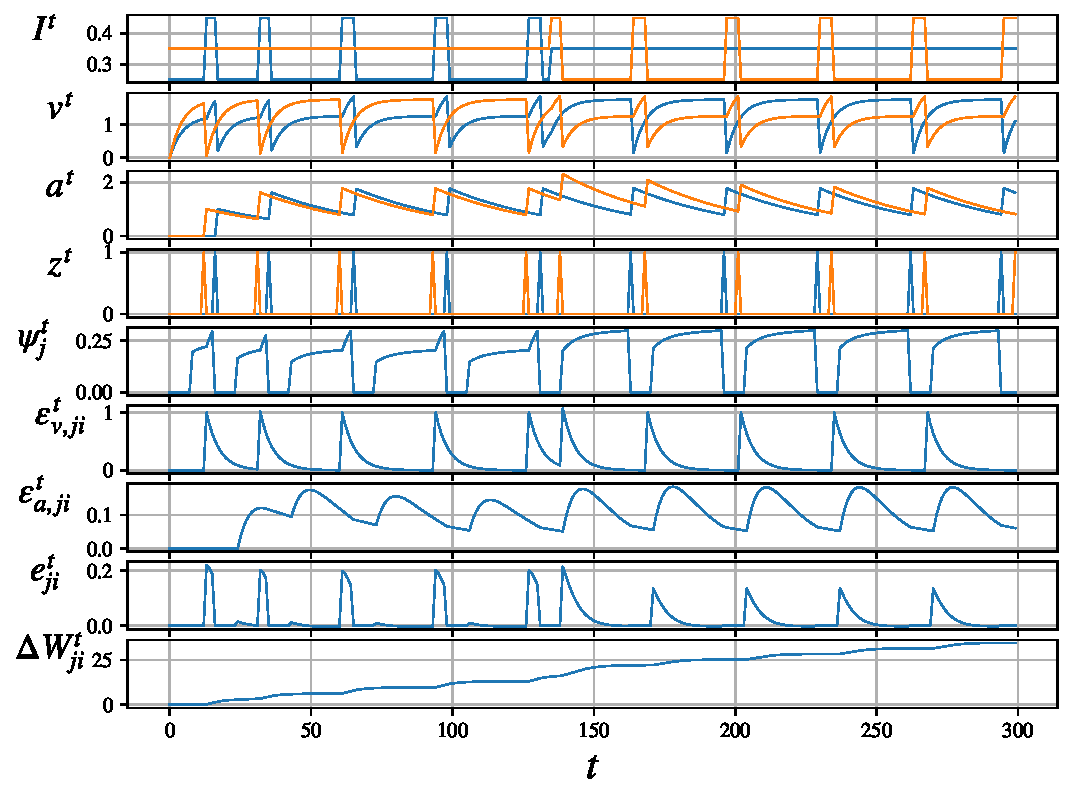
\includegraphics[width=\linewidth]{gfx/alif}
                \label{fig:alif}
                \caption[Single-synapse ALIF demo.]{A single-synapse demonstration of the evolution of the full hidden state of the ALIF neuron. The blue lines indicate the postsynaptic neuron $j$, and the orange lines indicate the presynaptic neuron $i$. Note that the synapse weight increases regardless of the order of spikes, indicating an absence of STDP in the standard e-prop ALIF neuron.}
            \end{figure}


